\documentclass{article} 
\usepackage{tikz-qtree}
\begin{document}
\pagenumbering{gobble}
\title{\bf{Academic Genealogical Tree}}
\author{Nicholas Malaya} \date{}
\maketitle
%
% [ s [.NP LaTeX ] [.VP [.V is ] [.NP fun ] ] 
%
%\Tree [.{Nicholas Penha Malaya, 2016} [.{Robert Delancey Moser Jr., 84}] ]
%\Tree [.{Nicholas Penha Malaya, 2016} [.NP LaTeX ] {test ing} ]
%
%\Tree [.{Nicholas Penha Malaya, 2016} [.{Robert Delancey Moser Jr., 1984} [.{Parviz Moin, 1978} [.{William Craig Reynolds, 1958} [.{William M. Kays, 1950} [.{Alexander Louis London, 1938} [.{Llewellen M. K. Boelter, 1918} [.{Gilbert Newton Lewis, 1899} {Theodore William Richards, 1888 (Nobel 1914)} ] ] ] ] [.{Stephen J. Kline, 1952} [.{Ascher H. Shapiro} {Joseph Henry Keenan} ] ] ] ] ] ]

\begin{center}
\resizebox{1.3\textwidth}{!}{%
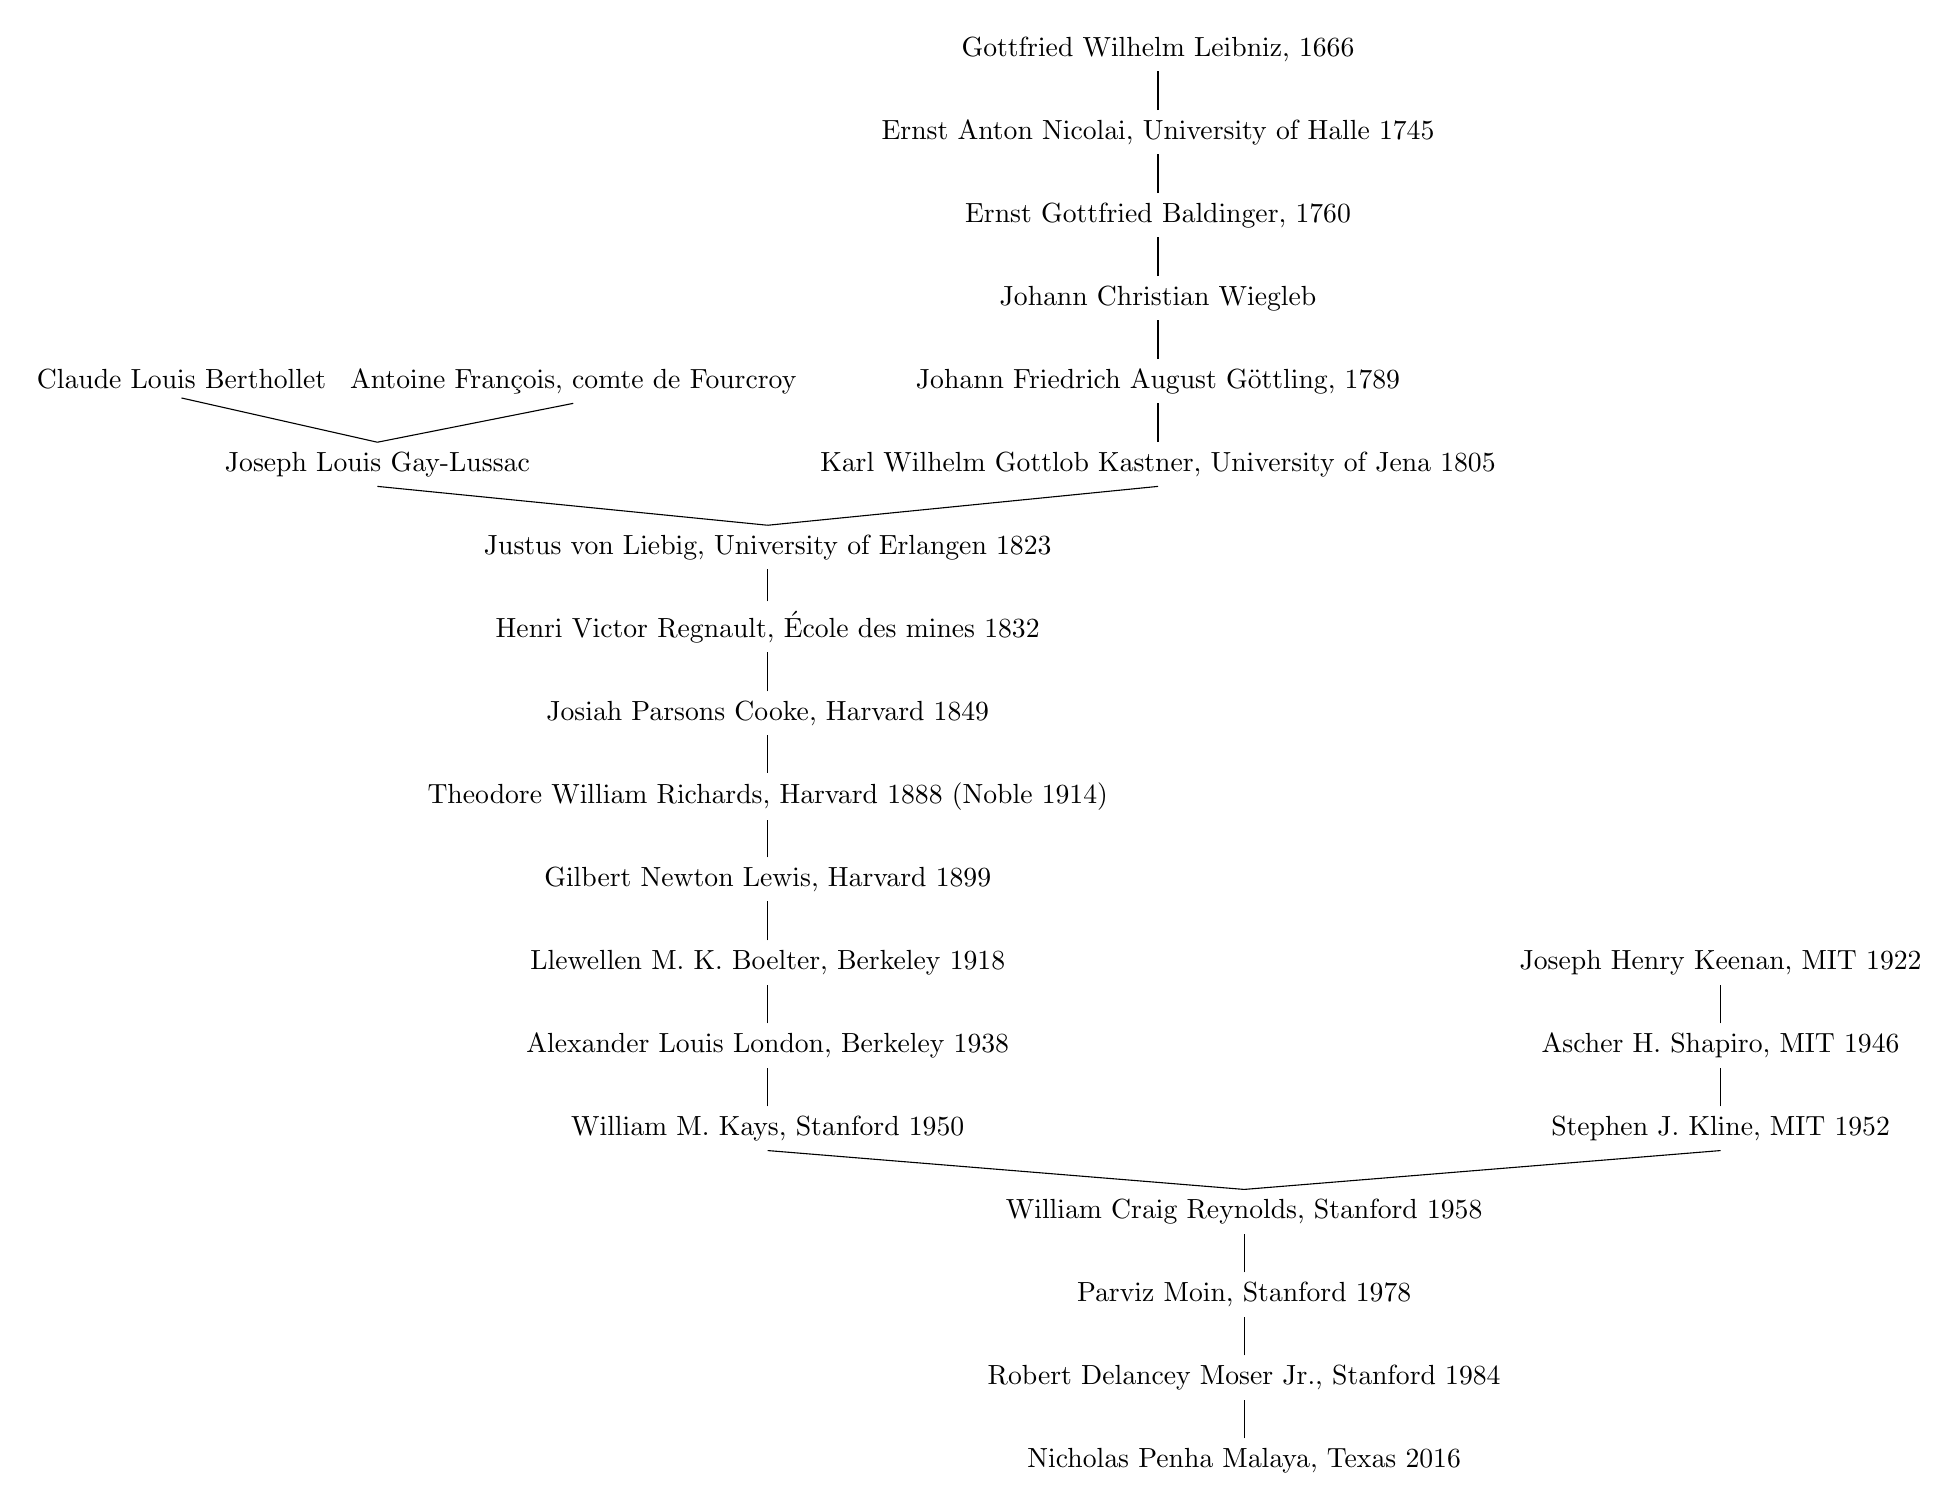
\begin{tikzpicture}[grow'=up]
\Tree [.{Nicholas Penha Malaya, Texas 2016} [.{Robert Delancey Moser Jr., Stanford 1984} [.{Parviz Moin, Stanford 1978} [.{William Craig Reynolds, Stanford 1958} [.{William M. Kays, Stanford 1950} [.{Alexander Louis London, Berkeley 1938} [.{Llewellen M. K. Boelter, Berkeley 1918} [.{Gilbert Newton Lewis, Harvard 1899} [.{Theodore William Richards, Harvard 1888 (Noble 1914)} [.{Josiah Parsons Cooke, Harvard 1849} [.{Henri Victor Regnault, \'Ecole des mines 1832} [.{Justus von Liebig, University of Erlangen 1823} [.{Joseph Louis Gay-Lussac} {Claude Louis Berthollet} {Antoine Fran\c{c}ois, comte de Fourcroy} ] [.{Karl Wilhelm Gottlob Kastner, University of Jena 1805} [.{Johann Friedrich August G\"ottling, 1789} [.{Johann Christian Wiegleb} [.{Ernst Gottfried Baldinger, 1760} [.{Ernst Anton Nicolai,  University of Halle 1745} {Gottfried Wilhelm Leibniz, 1666} ] ] ] ] ] ] ] ] ] ] ] ] ] [.{Stephen J. Kline, MIT 1952} [.{Ascher H. Shapiro, MIT 1946} {Joseph Henry Keenan, MIT 1922} ] ] ] ] ] ]
\end{tikzpicture}
}
\end{center}
\end{document}  

%
% http://genealogy.math.ndsu.nodak.edu/
%
% nick
% 10/14/16
%
